\chapter{Background}
%labels will help you to reference to certain images, tables, chapters, section, and so on...
\label{background}

%DELETEME: This chapter will cover all of your background information and related work. Background and related work are directly related to your thesis. Please do not place irrelevant content here which is a common mistake. Citing will be handled in the appendices.
%
%DELETEME: Background represents underlaying knowledge that is required to understand your work. The expected knowledge level of your readers can be set to the one of a bachelor or master student who just finished his studies (depending on what kind of thesis you are writing). This means that you do not need to describe how computers work, unless your thesis topic is about this. Everything that an avarage alumni from your field of studies should now does not need to be described. It turn, background information that is very complex and content-wise very near to you problem, can be placed in the main parts. Everyting else should be written here. Note: it is important to connect each presented topic to your thesis. E.g. if you present the ISO/OSI layer model you should also write that this is needed to understand the protocols you plan to develop in the main parts.
%
%DELETEME: Related work respresents results from work that handled the same or a similar problem that you are addressing. This work might have used a different approach or might not have been that successful. Finding a paper / work that solved your problem in the same way you were planning to do is not good and you should contact your supervizor for solving this issue. Again, each paper / work has to be connected to your approach: other papers might have not chosen an optimal solution; they might not have been taking care of essential aspects; they might have chosen a different approach and you believe, yours will work better ...

%###################################################################################
%###################### Topic A             ########################################
%###################################################################################
%\section{Topic 1}

%###################################################################################
%###################### Topic B             ########################################
%###################################################################################
\section{Imitation Learning with Dataset Aggregation} \label{sec:imitation_learning}

\newcommand{\parentheses}[1]{\left({#1}\right)}
\newcommand{\brackets}[1]{\left[{#1}\right]}
\newcommand{\braces}[1]{\left\{{#1}\right\}}

\newcommand{\timestep}{t}
\newcommand{\state}{\underline{x}}
\newcommand{\stateDomain}{\mathcal{X}}
\newcommand{\action}{\underline{u}}
\newcommand{\actionDomain}{\mathcal{U}}
\newcommand{\probability}{p}

\newcommand{\policy}{\pi}
\newcommand{\demonstration}{\xi}
\newcommand{\expertt}{*}
\newcommand{\parameterVector}{\underline{\theta}}
\newcommand{\trajectory}{\tau}

This section first, defines the general imitation learning problem, 
second, presents behavioral cloning as the simplest form of direct policy learning 
and third, introduces the more sophisticated direct policy learning method 
of dataset aggregation, 
which was originally proposed as DAgger by Ross et al. \cite{Ross2010}.
The experiments of this thesis (see chapter \ref{mainone}) 
dataset aggregation to the imitation learning problem 
of the ANN module in the autonomous navigation method (see chapter \ref{maintwo}). 



Imitation learning is an area of machine learning 
that considers the task of learning to
imitate (i.e., behave like) an expert 
in a sequential decision-making problem \cite{yue2018imitation}.
It applies naturally to learning problems where it is easier 
to demonstrate the desired behavior of how to attain a goal
than to define intermediate goals and rewards 
(as in supervised and reinforcement learning, respectively)
that lead to the desired behavior \cite{Nikolov2018}.
In terms of supervision,
imitation learning is therefore
between supervised learning
and reinforcement learning.
Imitation learning performs well in tasks
related to human intent or behavior, e.g.,
pedestrian avoidance \cite{Ziebart2009},
speech animation \cite{Taylor2017},
sport analytics \cite{le2017data}
and gaming \cite{thurau2004imitation}.
Regarding
planning and control
in autonomous navigation,
imitation learning has become 
state-of-the-art \cite{Mero2022}.
According to their approach, 
imitation learning methods 
divide into direct policy learning and 
inverse reinforcement learning \cite{RobotAutonomy2}.
Direct policy learning 
optimizes a policy class 
to approximate the expert's behavior
by reducing the imitation learning problem
to a single or a sequence of supervised learning problems.
Inverse reinforcement learning
optimizes a reward function 
to approximate the expert's underlying intent
and deploys reinforcement learning methods
to optimize a policy class to maximize the identified reward. 







\paragraph*{Problem Definition}$\ $\\
An imitation learning problem includes: 
a system, 
an expert, 
a policy class, 
a loss function, 
and a learning algorithm \cite{yue2018imitation}.
The goal is to find the policy 
within the policy class 
that approximates the expert's decision-making 
on the system's actions
as closely as possible. 

The system interacts with its real or simulated environment.
At time step $\timestep$,
the system is in the state $\state_\timestep \in \stateDomain$
and executes the action $\action_\timestep \in \actionDomain$
where $\stateDomain$ and $\actionDomain$ are the 
spaces of all existing system states and actions, respectively.
The system is considered a Markov decision process
whose initial state is randomly distributed 
%$\probability \parentheses{\state_0}$
\cite{RobotAutonomy2}.
Thus, a probabilistic transition model can 
describe the system dynamics 
providing the conditional probability distribution 
over the system state 
given the system state and action from the previous time step
\begin{align}
    \probability \parentheses{
        \state_\timestep | \state_{\timestep -1}, \action_{\timestep -1}
    }.
\end{align}

%Note that the explicit system dynamics are typically unknown 
%for the policy class to be trained.

The expert 
%(also referred to as demonstrator)
is a human or a computer program 
that makes state-based action decisions,
which cause the system to act as desired.
The expert policy, which maps system states to expert actions, 
represents the expert's decision-making process
\begin{align}
    \policy^\expertt
    :\ \stateDomain \rightarrow \actionDomain
    ;\quad 
    \state_\timestep 
    \mapsto 
    \action_\timestep^\expertt
    %\policy^\expertt\parentheses{\state_\timestep}
    .
\end{align}
Applying the expert policy on a system state
yields a demonstration,
i.e., a state-action pair 
$\parentheses{\state_\timestep, \action_\timestep^\expertt}$.


The policy class defines the search space for
finding the optimal policy, i.e., 
the policy that most closely resembles the expert policy.
Usually, 
the policy class is an ANN
\begin{equation}
    \policy_{\parameterVector}
    :\ \stateDomain \rightarrow \actionDomain
    ;\quad \state_\timestep \mapsto 
    \policy_{\parameterVector} \parentheses{\state_\timestep}
\end{equation}
where the vector $\parameterVector$ 
contains the trainable parameters of the ANN.

Both, the expert policy 
and members of the policy class, can roll out.
%Rolling out the expert policy
%yields a trajectory of demonstrations
%$\trajectory = \parentheses{\state_\timestep, \action_\timestep^\expertt}
%_{\timestep \in \braces{0, 1, \dots}}$.
The rollout of a general policy 
$\policy :\ \stateDomain \rightarrow \actionDomain$
denotes the process, 
in which the system, 
starting from the initial state 
$\state_0 \sim \probability \parentheses{\state_0}$,
interacts with the environment 
based on the actions inferred by that policy
for a certain number of time steps
\begin{align}
    \probability \parentheses{
        \state_\timestep | \state_{\timestep -1}, \policy\parentheses{\state_{\timestep-1}}
    },\ \timestep \in \braces{0,\dots, T}.
\end{align}
A rollout produces a trajectory,
which is the sequence of the state-action pairs visited during rollout
\begin{align}
    \trajectory = \parentheses{\state_\timestep, 
    \policy\parentheses{\state_\timestep}}
    _{\timestep \in \braces{0, \dots, T}}.    
\end{align}
The policy induces the state distribution of a rollout, i.e., the probability that the system visits a state, which would therewith become part of the rollout trajectory. The rollout state distribution is the average of the state distributions over the time steps of the rollout.
\begin{equation}
    \probability \parentheses{\state | \policy}
    = \frac{1}{T+1} \sum_{\timestep = 0}^T
    \probability \parentheses{\state_\timestep | \policy}.
\end{equation}


%Multiple expert trajectories constitute a training dataset
%%on which the policy class can be trained
%\begin{align}
%    D = \braces{\trajectory_i}_{i \in \braces{1, 2, \dots}}.
%\end{align}


%The rollout of a member of the policy class also produces
%a trajectory ...
%The policy class can be rolled out, i.e.,
%to repeatedly apply the policy on an inital state.
%Thereby, it generates the trajectory 
%\begin{align}
%    \tau = \braces{
%        \parentheses{\state_\timestep, \policy \parentheses{\state_\timestep}}
%    }_{\timestep \in \braces{0, 1, \dots}}
%    .
%\end{align}
The loss function measures
how much an action 
predicted by a policy for a system state
deviates
from the action demonstrated by the expert for the same state
\begin{align}
    L_{\policy}
    :\ \stateDomain \rightarrow \mathbb{R}
    ;\quad
    \state_\timestep
    \mapsto
    L_{\policy}
    \parentheses{
        \policy\parentheses{\state_\timestep},
        \policy^\expertt\parentheses{\state_\timestep}
    }.
\end{align}
Applied on a set of demonstrations,
the loss function quantifies how closely a policy
imitates the expert policy. 



%The learning algorithm 
%finds the policy $\hat{\policy}^\expertt$ 
%within the policy class 
%that is closest to the expert policy. 
%For this purpose, the algorithm 
%minimizes the total imitation loss 
%evaluated on states sampled 
%from the distribution 
%induced by the identified policy itself.
%In machine learning, 
%this corresponds to the training of the ANN, 
%whereby the algorithm updates the trainable parameters of the ANN 
%in accordance to the evaluated loss

The learning algorithm searches for the optimal policy 
$\hat{\policy}^\expertt$
within the policy class by minimizing the total imitation loss, 
whereby the state distribution of the loss evaluation 
is equal to the distribution when rolling out the optimal policy.
As a result, the state distributions at learning and test rollouts 
do not differ, which ensures that low training losses 
transfer to high test performances.
In machine learning, this corresponds to the training of the ANN, 
in which the algorithm updates the trainable parameters of the ANN 
in accordance to the evaluated loss
\begin{equation}
    \hat{\policy}^\expertt
    =
    \argmin{\parameterVector}
    \sum_{
        \state \sim \probability \parentheses{
            \state | \policy_{\parameterVector}}
    }
    L_{\policy_{\parameterVector}} \parentheses{\state}
    %L \parentheses{
    %    \policy_{\parameterVector}\parentheses{\state_\timestep},
    %    \policy^\expertt\parentheses{\state_\timestep}
    %}
    .
\end{equation}
The above optimization is a 
``non-i.i.d. supervised learning problem" \cite{Ross2010}. 
As the system dynamics are unknown or too complex, 
training data can only be collected in rollouts. 
Thereby, the distribution of the training data is induced 
by the rolled out policy and hence 
neither independent and identically distributed (i.i.d.) 
across the system state space $\stateDomain$ 
nor equal to the distribution 
induced by the optimal policy yet unknown. 
Because of the interdependence of policies and training data distributions, 
closing the ``distributional mismatch" \cite{RobotAutonomy2} 
is a non-convex optimization problem, 
which is significantly more difficult and time-consuming 
than common supervised learning.





\paragraph*{Behavioral Cloning}$\ $\\
Behavioral cloning reduces the imitation learning problem 
to a single, convex supervised learning problem 
on a pre-collected training dataset 
of expert trajectories, where each trajectory is the product of an 
expert policy rollout and 
contains the thereby demonstrated state-action pairs
\begin{equation}
    D = \braces{\trajectory_i^\expertt}_{i \in \braces{1, 2, \dots}}
    ,\quad
    \trajectory_i^\expertt = \parentheses{
        \state_{i,\timestep}, \action_{i,\timestep}^\expertt}
    _{\timestep \in \braces{0, 1, \dots}}.
\end{equation}
The optimization problem of behavioral cloning
is to minimize the 
total imitation loss on the demonstrations
$\parentheses{\state_\timestep, \action_\timestep^\expertt}$ 
in the trajectories 
$\trajectory_i$
of the pre-collected dataset $D$
\begin{align}
    \hat{\policy}^\expertt
    &=
    \argmin{\parameterVector}
    \sum_{\trajectory_i \in D} \quad
    \sum_{\parentheses{\state_\timestep, \action_\timestep^\expertt} \in \trajectory_i
    }
    L \parentheses{
        \policy_{\parameterVector} \parentheses{\state_\timestep},
        \action_\timestep^\expertt
    }
    \nonumber\\ &=
    \argmin{\parameterVector}
    \sum_{
        \state \sim \probability \parentheses{
            \state | \policy^\expertt}
    }
    L_{\policy_{\parameterVector}} \parentheses{\state}
    ,
\end{align}
given the expert rollout state distribution
\begin{equation}
    \probability \parentheses{\state | \policy^\expertt}
    = \frac{1}{T+1} \sum_{\timestep = 0}^T
    \probability \parentheses{\state_\timestep | \policy^\expertt}.
\end{equation}
Compared to general imitation learning, behavioral cloning 
generally exhibits different distributions at training and testing
\begin{equation}
    \probability \parentheses{\state | \policy^\expertt}
    \neq 
    \probability \parentheses{\state | \policy_{\parameterVector}}.
\end{equation}
This plus the fact that the training data is 
generally not i.i.d. across the state space 
makes it likely that the ANN, when rolling out, 
faces states not seen during training. 
As a result, low training losses do not guarantee high test performances. 
This is especially true for a longer rollouts 
because the upper bound of the error grows quadratically 
with the number of time steps $T$ \cite{yue2018imitation}. 
Although the above optimization minimizes 
the one-step loss of the ANN along the expert trajectories, 
when the ANN rolls out, these one-step errors accumulate 
along the ANN trajectory and will very likely 
cause non-negligible deviations from the expert trajectories 
of the training dataset.




\paragraph*{Dataset Aggregation}$\ $\\
Dataset aggregation (originally proposed as DAgger \cite{Ross2010}) 
extends behavioral cloning iteratively.
It reduces the imitation learning problem 
to a sequence of convex supervised learning problems.
The fundamental concept of the method takes the following steps.
\begin{enumerate}
    \item 
    Roll out the expert policy $\policy^\expertt$,
    record the thereby resulting trajectory
    and initialize the aggregated dataset with that trajectory
    $D_0 = \trajectory_0$.
    Train the ANN with supervised learning on the aggregated dataset
    to receive
    $\policy_{\parameterVector, 0}$.
    \item Until the ANN exhibits the desired behavior when rolling out, 
    do for iteration $i = 1,2,\dots$
    \begin{enumerate}
        \item Rollout the ANN from the last training
        $\policy_{\parameterVector, i-1}$
        and record the thereby visited states
        $\parentheses{\state_{i,\timestep}}_{t\in \braces{0, \dots, T_i}}$.
        \item Apply the expert policy to the recorded states 
        to receive a trajectory of demonstrations
        $\trajectory_i = \parentheses{\state_{i,\timestep}, 
    \policy^\expertt\parentheses{\state_{i,\timestep}}}
    _{\timestep \in \braces{0, \dots, T_i}}$.
        \item Add the labeled trajectory to the aggregated dataset
        $D_i = D_{i-1} \cup \trajectory_i$.
        \item Train the ANN with supervised learning on the aggregated dataset
        to receive
        $\policy_{\parameterVector, i}$.
    \end{enumerate}
\end{enumerate}
In contrast to behavioral cloning,
dataset aggregation requires first, 
access to the system for executing ANN rollouts
and second, 
an interactive expert providing feedback 
on the thereby visited states \cite{yue2018imitation}.
In the iterative learning process,
dataset aggregation
remembers and confronts the ANN with
its mistakes made in rollouts corrected by the expert.
Ideally, this procedure reduces the 
state distribution differences between learning and rollouts
to the point where
the trainable parameters of the ANN converge to their
optimal values for the general imitation learning problem.





%###################################################################################
%###################### Topic C             ########################################
%###################################################################################
\section{Gated Recurrent Unit} \label{sec:gru}
In this thesis,
the ANN module of the autonomous navigation method (see section \ref{mainone})
is extended with the gated recurrent unit (GRU), 
which is a special recurrent neural network (RNN) architecture
proposed by Cho et al. \cite{Cho2014},
with the aim to involve temporal comprehension in
the navigation decision-making.
This section introduces the class of RNNs
and relates the GRU to standard RNNs
and the more prevalent long short-term memory (LSTM).
Moreover, it provides information regarding first,
the state and gating mechanisms that make the GRU able to comprehend temporally at inference
and second, how the GRU learns with backpropagation through time.

\paragraph*{Recurrent Neural Networks} ${}$\\
RNNs contrasts with classical feedforward ANNs, 
which forward information only towards subsequent layers, 
by featuring dynamic properties that stem 
from implementing feedback connections
\cite{Hu2008} (see fig. \ref{fig:rnn_folded}).
As previously inferred states re-enter the network, 
the output of an RNN depends not only on the current 
but also on prior inputs. 
In this sense, RNNs are qualified to process and infer from 
entire sequences of data points. 
In the case of time-series data, 
this equates to temporal comprehension and memory \cite{ICE2020}.
RNNs train on sequential data with backpropagation through time (BPTT) 
\cite{pascanu2013difficulty}
which is basically the application of standard backpropagation
(e.g., \cite{Rojas1996})
on the unfolded representation of an RNN
(see fig. \ref{fig:rnn_unfolded}).
This representation exhibits a layer 
for each data point in the processed input sequence 
and is construable as a feedforward ANN 
that shares its trainable parameters across its layers. 
The longer the input sequences,
the deeper the unfolded representation of an RNN becomes. 
The training of RNNs on long input sequences 
is hence prone to the 
vanishing gradient problem \cite{hochreiter1991untersuchungen},
which slows down or ceases the convergence 
of the trainable parameters of the RNN.
As a result, standard RNNs have difficulties 
learning to connect to information deep in the past \cite{Bengio1994}.
\begin{figure}[h]
    \centering
    \subfloat[
        Folded
    ]{
        \label{fig:rnn_folded}
        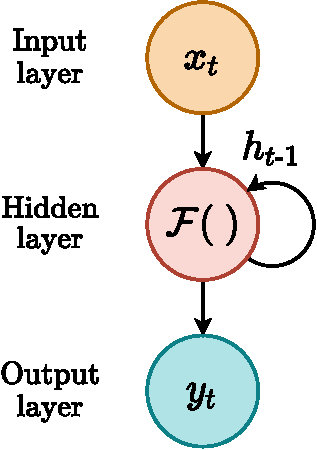
\includegraphics[height=0.35\textwidth]{own/rnn_folded.drawio.pdf}
    }
    \hspace*{2cm}                
    \subfloat[
        Unfolded
    ]{
        \label{fig:rnn_unfolded}
        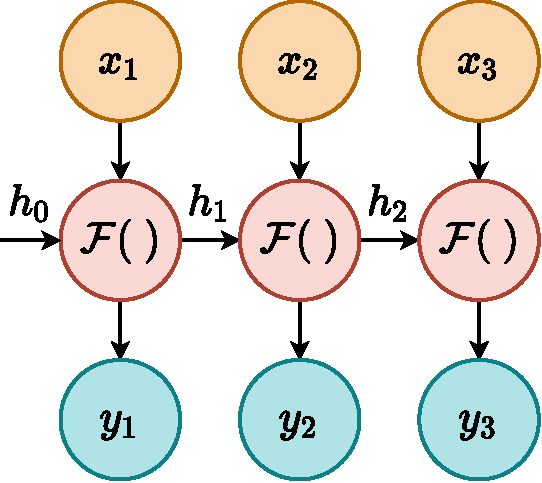
\includegraphics[height=0.35\textwidth]{own/rnn_unfolded.drawio.pdf}
    }
    \caption[
        Folded and unfolded RNN
    ]{
        Folded representation of an RNN with a single hidden layer 
        inferring $y_t = \mathcal{F}\left(x_t, h_{t-1}\right)$ from the current input
        and the previous hidden state
        and the time-unfolded representation
        when processing the input sequence
        $\left(x_i\right)_{i\in\{1, 2, 3\}}$.
        \label{fig:rnn_folded_unfolded}
    }
\end{figure}




In 1997, Hochreiter and Schmidhuber \cite{Hochreiter1997} 
introduced the long short-term memory (LSTM), 
which is today's predominant RNN architecture \cite{schmidhuber_2021}. 
A standard LSTM layer
recurrently maintains a cell state and a hidden state. 
This means that, besides the current data point of the input sequence, 
the layer re-inputs the fed back cell state and hidden state 
from the previous sequential step. 
Furthermore, the LSTM layer implements three gating mechanisms 
to control the information flow within the layer. 
A gating mechanism is basically the Hadamard product 
of a state and a gate, 
which is a vector whose entries are within the interval from zero to one. 
Consequently, a gate applied to a state controls the flow 
of the state elements within the range from zero to full flow. 
The forget gate of the LSTM layer controls the flow 
from the previous to the current cell state. 
The input gate controls the flow from the previous hidden state 
and the current data point of the input sequence 
to the current cell state. 
And the output gate controls the flow from the current cell state 
to the current hidden state. 
By this design of recurrent states with gated information flow, 
the training of the LSTM is essentially robust 
to the vanishing gradient problem \cite{pascanu2013difficulty}. 
As a result, the LSTM is, compared to standard RNNs, 
more capable of learning to remember long-term dependencies 
within input sequences.


The GRU, which was proposed 17 years after the LSTM by 
Cho et al. \cite{Cho2014}, 
is a lighter version of the LSTM. 
It refrains from the cell state and therewith the output gate of the LSTM 
and only has a hidden state and two gating mechanisms. 
Therewith, the GRU has less trainable parameters 
than the LSTM and is less memory efficient. 
Nevertheless, it preserves the robustness towards 
the vanishing gradient problem \cite{ICE2020}. 
Various empirical studies compared the GRU and the LSTM. 
Greff et al. \cite{Greff2017} found no substantial performance 
differences between the GRU and several LSTM variants 
in speech and handwritten text recognition and music representation. 
Chung et al. \cite{Chung2014} detected an equally well performance 
of the GRU and the LSTM processing raw speech and polyphonic music data. 
In the comparative study of Yin et al. \cite{Yin2017}, 
the GRU slightly outperforms the LSTM 
in five of seven natural language processing tasks. 
Kaiser and Sutskever \cite{Kaiser2015} achieved better 
results with a GRU-based than with an LSTM-based network 
in algorithm learning. 
Considering the above findings and the lower complexity, 
this thesis uses the GRU and not the LSTM 
for the ANN module of the autonomous navigation method.




\paragraph*{Inference}$\ $\\
The following presents the mathematics 
of the inference
of a single GRU layer
in accordance with the PyTorch implementation\footnote{
    \url{https://pytorch.org/docs/stable/generated/torch.nn.GRU.html}, accessed on \today
}.
This includes the layer's two gating mechanisms
and its computations of the candidate state and the hidden state.






Without loss of generality,
let the sequential data to be processed by the GRU layer
be a batch of time series of data points
\begin{equation}
    \left(
        \underline x_t
        \in \mathbb{R}^{N^\text{in}}
    \right)_{
        t \in \left\{
            1, \dots, N^\text{seq}
        \right\}
        ,
        i
    }
    ,\quad
    i \in \left\{
        1, \dots, N^\text{batch}
    \right\},
\end{equation}
where $N^\text{batch}$ is the batch size, 
$N^\text{seq}$ is the sequence length 
and $N^\text{in}$ is the dimensionality of the data points.
Let the initial batch of hidden states be
\begin{equation} \label{eq:gru_init_hidden_state}
    \underline h_{0,i}
    \in \left[-1, 1\right]^{N^\text{hidden}}
    ,\quad
    i \in \left\{
        1, \dots, N^\text{batch}
    \right\},
\end{equation}
where $N^\text{hidden}$ is the dimensionality
of the hidden state, which is a design parameter of the GRU layer.
The values of the initial hidden states $\underline h_{0,i}$
are typically zero or noisy \cite{Zimmermann2012}
but can also be learned (e.g., \cite{Forcada1995}).
The GRU layer processes the time series included in the batch parallelly 
and the data points of the individual time series successively.
At the current time step $t$,
the layer's input comprises 
the batch of the current data points
and the fed back batch of previously outputted, hidden states
\begin{equation}
    \left(
    \underline x_{t,i}
    ,\ 
    \underline h_{t-1,i}
    \right)
    ,\quad
    i \in \left\{
        1, \dots, N^\text{batch}
    \right\}.
\end{equation}
For simplification, the following text only refers 
to the parallelly computed, individual elements of the processed batch. 
However, the following equations yet explicitly refer to the entire batch.


At every incoming input, the GRU layer initially computes its two gates. 
The current reset gate 
\begin{equation}
    \underline g^\text{r}_{t,i} 
    =
    \mathcal{F}^\text{r} \left( \underline x_{t,i}, \underline h_{t-1,i}\right)
    ,\quad i \in \left\{1, \dots, N^\text{batch}\right\}
\end{equation}
results from the map
\begin{align} \label{eq:gru_reset}
    \mathcal{F}^\text{r}
    &:
    \left(\mathbb{R}^{N^\text{in}},\ \left[-1, 1\right]^{N^\text{hidden}}\right)
    \rightarrow
    \left[0, 1\right]^{N^\text{hidden}}
    \nonumber \\ & \quad
    \left(\underline x,\underline h\right)
    \mapsto
    \hadfct{\sigma} \left(
        \underline{\underline A}^\text{r}_{x} \underline x
        +
        \underline b^\text{r}_{x}
        +
        \underline{\underline A}^\text{r}_{h} \underline h
        +
        \underline b^\text{r}_{h}
    \right).
\end{align}
The above map to the reset gate comprises two steps. 
First, it linearly transforms the current data point 
and the previous hidden state 
with the trainable weight matrices and bias vectors
\begin{align} \label{eq:gru_reset_params}
    \underline{\underline A}^\text{r}_{x} & \in \mathbb{R}^{
        N^\text{hidden}
        \times
        N^\text{in}
    },
    & \underline{b}^\text{r}_{x} & \in \mathbb{R}^{N^\text{hidden}},
    \nonumber \\
    \underline{\underline A}^\text{r}_{h} & \in \mathbb{R}^{
        N^\text{hidden}
        \times
        N^\text{hidden}
    },
    & \underline{b}^\text{r}_{h} & \in \mathbb{R}^{N^\text{hidden}},
\end{align}
whereby the user has the design option to disable all biases of the GRU layer.
This is tantamount to set the above and the below biases of the layer to zero 
and consider them not trainable.
Second, the standard sigmoid function \cite{Han1995} 
(see fig. \ref{fig:gru_activations})
\begin{equation} \label{eq:sigmoid}
    \sigma :\ 
    \mathbb{R} \rightarrow \left[0,1\right] ;\ 
    x \mapsto \frac{1}{1 + e^{-x}}
\end{equation}
applies element-wise (denoted with the accent $\odot$) 
to the sum of these two linear transformations.
The sigmoid function limits the values of the reset gate 
to the interval between zero and one. 
This is characteristic of a gating mechanism, 
which targets at only damping, 
not amplifying or reversing the individual values of the state.

The current update gate 
\begin{equation}
    \underline g^\text{u}_{t,i} 
    =
    \mathcal{F}^\text{u} \left( \underline x_{t,i}, \underline h_{t-1,i}\right)
    ,\quad i \in \left\{1, \dots, N^\text{batch}\right\}
\end{equation}
results from the map
\begin{align} \label{eq:gru_update}
    \mathcal{F}^\text{u}
    &:
    \left(\mathbb{R}^{N^\text{in}},\ \left[-1, 1\right]^{N^\text{hidden}}\right)
    \rightarrow
    \left[0, 1\right]^{N^\text{hidden}}
    \nonumber \\ & \quad
    \left(\underline x,\underline h\right)
    \mapsto
    \hadfct{\sigma} \left(
        \underline{\underline A}^\text{u}_{x} \underline x
        +
        \underline b^\text{u}_{x}
        +
        \underline{\underline A}^\text{u}_{h} \underline h
        +
        \underline b^\text{u}_{h}
    \right).
\end{align}
The above map to the update gate is the same 
as the map to the reset gate but has 
its own trainable weight matrices and bias vectors
\begin{align} \label{eq:gru_update_params}
    \underline{\underline A}^\text{u}_{x} & \in \mathbb{R}^{
        N^\text{hidden}
        \times
        N^\text{in}
    },
    & \underline{b}^\text{u}_{x} & \in \mathbb{R}^{N^\text{hidden}},
    \nonumber \\
    \underline{\underline A}^\text{u}_{h} & \in \mathbb{R}^{
        N^\text{hidden}
        \times
        N^\text{hidden}
    },
    & \underline{b}^\text{u}_{h} & \in \mathbb{R}^{N^\text{hidden}}.
\end{align}

Knowing the current reset gate, the GRU layer computes the candidate state
\begin{equation}
    h^\text{c}_{t,i}
    =
    \mathcal{F}^\text{c} \left( \underline x_{t,i}, \underline h_{t-1,i}\right)
    ,\quad i \in \left\{1, \dots, N^\text{batch}\right\}
\end{equation}
with the map
\begin{align} \label{eq:gru_candidate}
    \mathcal{F}^\text{c}
    &:
    \left(
        \mathbb{R}^{N^\text{in}}, \left[-1, 1\right]^{N^\text{hidden}}
    \right)
    \rightarrow
    \left[-1, 1\right]^{N^\text{hidden}}
    \nonumber \\ & \quad
    \left(\underline x, \underline h \right)
    \mapsto
    \hadfct{\tanh} \left[
        \underline{\underline A}^\text{c}_{x}
        \underline x
        +
        \underline b^\text{c}_{x}
        +
        \mathcal{F}^\text{r} \left(\underline x, \underline h \right)
        \odot
        \left(
            \underline{\underline A}^\text{c}_{h}
            \underline h
            +
            \underline b^\text{c}_{h}
        \right)
    \right],
\end{align}
which has the trainable weight matrices and bias vectors
\begin{align} \label{eq:gru_candidate_params}
    \underline{\underline A}^\text{c}_{x} & \in \mathbb{R}^{
        N^\text{hidden}
        \times
        N^\text{in}
    },
    & \underline{b}^\text{c}_{x} & \in \mathbb{R}^{N^\text{hidden}},
    \nonumber \\
    \underline{\underline A}^\text{c}_{h} & \in \mathbb{R}^{
        N^\text{hidden}
        \times
        N^\text{hidden}
    },
    & \underline{b}^\text{c}_{h} & \in \mathbb{R}^{N^\text{hidden}}.
\end{align}
The above map to the candidate state 
resembles the maps to the reset and the update gate 
by subjecting the current data point and the previous hidden state 
to a separate, biased linear transformation, 
but differs in two aspects. 
First, before adding the results of the two transformations, 
the current reset gate applies to the transformed, previous hidden state 
($\odot$ denotes the Hadamard product).
Thereby, the reset gate mitigates the contribution 
of the previous hidden state to the candidate state. 
Second, instead of the sigmoid function, 
the hyperbolic tangent \cite{D.1966} (see fig. \ref{fig:gru_activations})
\begin{equation} \label{eq:tanh}
    \tanh
    :\ 
    \mathbb{R}
    \rightarrow
    \left[
        -1,1
    \right]
    ;\ 
    x 
    \mapsto 
    \frac{
        e^x - e^{-x}
    }{
        e^x + e^{-x}
    }
\end{equation}
applies element-wise to the sum of the transformed data point 
and the gated, transformed, previous hidden state, 
which limits the values of the candidate state 
to the interval from minus to plus one.



Finally, the GRU layer computes the current hidden state
\begin{equation} \label{eq:gru_layer_current_hidden}
    h_{t,i}
    =
    \mathcal{F}^\text{h} \left( \underline x_{t,i}, \underline h_{t-1,i}\right)
    ,\quad i \in \left\{1, \dots, N^\text{batch}\right\}
\end{equation}
with the map
\begin{align} \label{eq:gru_layer_map_hidden}
    \mathcal{F}^\text{h}
    &:
    \left(
        \mathbb{R}^{N^\text{in}}
        ,\ 
        \left[-1, 1\right]^{N^\text{hidden}}
    \right)
    \rightarrow
    \left[-1, 1\right]^{N^\text{hidden}}
    \nonumber \\ & \quad
    \chi := \left(
        \underline x
        ,\ 
        \underline h
    \right)
    \mapsto 
    %\dots \nonumber \\ & \qquad \qquad \dots
    \left[
        \underline 1 
        -
        \mathcal{F}^\text{u}\left(\chi\right)
    \right]
    \odot
    \mathcal{F}^\text{c} \left(\chi\right)
    +
    \mathcal{F}^\text{u}\left(\chi\right)
    \odot
    \underline h
    .
\end{align}
The above map to the hidden state is a weighted arithmetic mean 
of the previous hidden state and the current candidate state, 
where the current update gate and its counter gate are the weights. 
Therewith, the update gate controls the element-wise percentages 
of the two states in the current hidden state. 
The fact that the hyperbolic tangent normalizes the elements 
of the candidate state to the interval from minus to plus one 
(see equ. \ref{eq:gru_candidate})
limits the values of the current hidden state to the same interval 
(given that the values of initial hidden state
(equ. \ref{eq:gru_init_hidden_state})
are also in that interval).
\begin{figure}
    \centering
    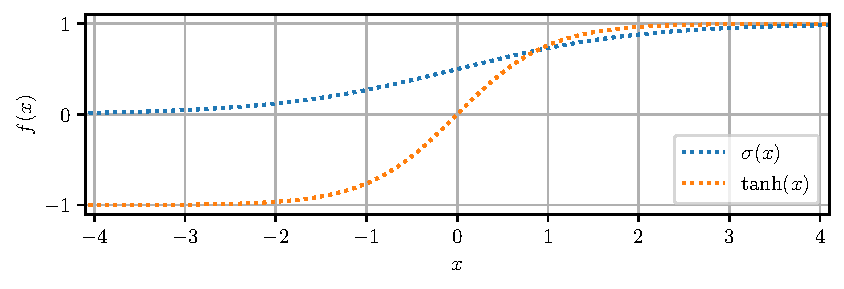
\includegraphics[width=0.9\textwidth]{own/sigmoid_tanh.pdf}
    \caption[
        Activation functions of the GRU
    ]{
        Activation functions of the GRU.
        The standard sigmoid function
        (see equ. \ref{eq:sigmoid})
        normalizes the values
        of the reset and the update
        gate to the interval from zero to one
        (see equ. \ref{eq:gru_reset} and \ref{eq:gru_update}).
        The hyperbolic tangent
        (see equ. \ref{eq:tanh})
        normalizes the values 
        of the candidate
        and therewith the hidden state 
        to the interval from minus to plus one
        (see equ. \ref{eq:gru_candidate} and \ref{eq:gru_layer_map_hidden}).
        \label{fig:gru_activations}}
\end{figure}




\paragraph*{Backpropagation through Time}$\ $\\
The following illustrates backpropagation through time (BPTT) 
applied to a single integrated GRU layer, 
which operates in many-to-one mode. 
BPTT calculates the gradients of the loss with respect to the 
trainable parameters of the GRU. 
Learning algorithms update the trainable parameters 
based on these gradients to minimize the loss.

%During training,
%the integrated GRU layers 
%of the ANN module of the navigation method of this thesis
%run in many-to-one mode,
%i.e., sequential inputs are mapped to single outputs \cite{ICE2020}.
%The trainable weights of the ANN module
%are updated with gradient-based methods 
%that minimize the loss.
%These gradient-based methods require 
%the knowledge of the gradient of the loss 
%with respect to the ANN's trainable parameters.
%The following paragraph shows the computation of these gradients 
%with backpropagation through time for 
%an integrated GRU layer in many-to-one mode.




%During the training of the ANN module 
%of the navigation method of this thesis
%(see section \ref{sec:ann_module}),
%the GRU sub-module,
%which integrates multiple, subsequent GRU layers,
%operates in many-to-one mode,
%i.e., the map of sequential inputs to single outputs.
%The following provides the theoretical
%background of training a single GRU layer in many-to-one mode.



%During the testing of the navigation method,
%the GRU layers of the ANN module operate 
%in one-to-one mode,
%i.e., a single input is mapped to a single output.
%At a high frequency,
%each incoming single data point,
%containing the current data from onboard sensors, 
%is mapped to a single navigation decision.
%During the training of the ANN module,
%on the contrary,
%the GRU layers process many-to-one,
%i.e., sequential input is mapped to a single output.
%The training data consist of sequences
%of data points labeled with a single navigation decision.
%The output of the gru layers is hence
%not the whole sequence of hidden states 
%but only the last inferred hidden state of a sequence.
%This last hidden state is then forwarded
%through the remaining layers of the ANN module.
%Then,
%the final output of the ANN module
%is related with the label of the sequence
%in order to compute the loss.
%To update the weights of the network after an batch
%the loss is backpropagated.

Let a single GRU layer, integrated into a superordinate ANN, o
perate in many-to-one mode. 
Given biases enabled, the set of all objects of trainable parameters is
\begin{equation} \label{eq:gru_params}
    \Theta 
    = 
    \left\{  
        \underline{\underline A}^\text{r}_{x},
        \underline{b}^\text{r}_{x},
        \underline{\underline A}^\text{r}_{h},
        \underline{b}^\text{r}_{h},
        \underline{\underline A}^\text{u}_{x},
        \underline{b}^\text{u}_{x},
        \underline{\underline A}^\text{u}_{h},
        \underline{b}^\text{u}_{h},
        \underline{\underline A}^\text{c}_{x},
        \underline{b}^\text{c}_{x},
        \underline{\underline A}^\text{c}_{h},
        \underline{b}^\text{c}_{h}
    \right\}
\end{equation}
(see equ. \ref{eq:gru_reset_params},
\ref{eq:gru_update_params} 
and \ref{eq:gru_candidate_params}).
The total number of trainable parameters of the GRU layer is
\begin{align} \label{eq:gru_layer_nparams}
    N^\text{param} 
    = 
    \begin{cases}
        3 N^\text{hidden} \left(
            N^\text{in}
            + N^\text{hidden}
            + 2
        \right)
        ,\ 
        & \text{if biases enabled} \\
        3 N^\text{hidden} \left(
            N^\text{in}
            + N^\text{hidden}
        \right)
        ,\ 
        & \text{else}.
    \end{cases}
\end{align}
At a single inference, the GRU layer inputs a 
batch of sequences of feature vectors from the precedent layer of the ANN
\begin{equation}
    \left(\underline x_t\right)_{t\in\{1,\dots,N^\text{seq}\},i}
    , \quad i \in \left\{1,\dots,N^\text{batch}\right\}.
\end{equation}
The GRU layer maps each incoming batch of sequences 
to a batch of single outputs, 
whereby a single output is the hidden state 
from the last processing step in the sequence
\begin{equation} \label{equ:gru_output_many_to_one}
    \underline y_i = \underline h_{N^{seq}, i},
    \quad i \in \left\{1,\dots,N^\text{batch}\right\}.
\end{equation}
Figure \ref{fig:gru_unfolded} shows the time-unfolded computation graph 
of the integrated GRU layer for a single batch element.
\begin{figure}
    \centering
    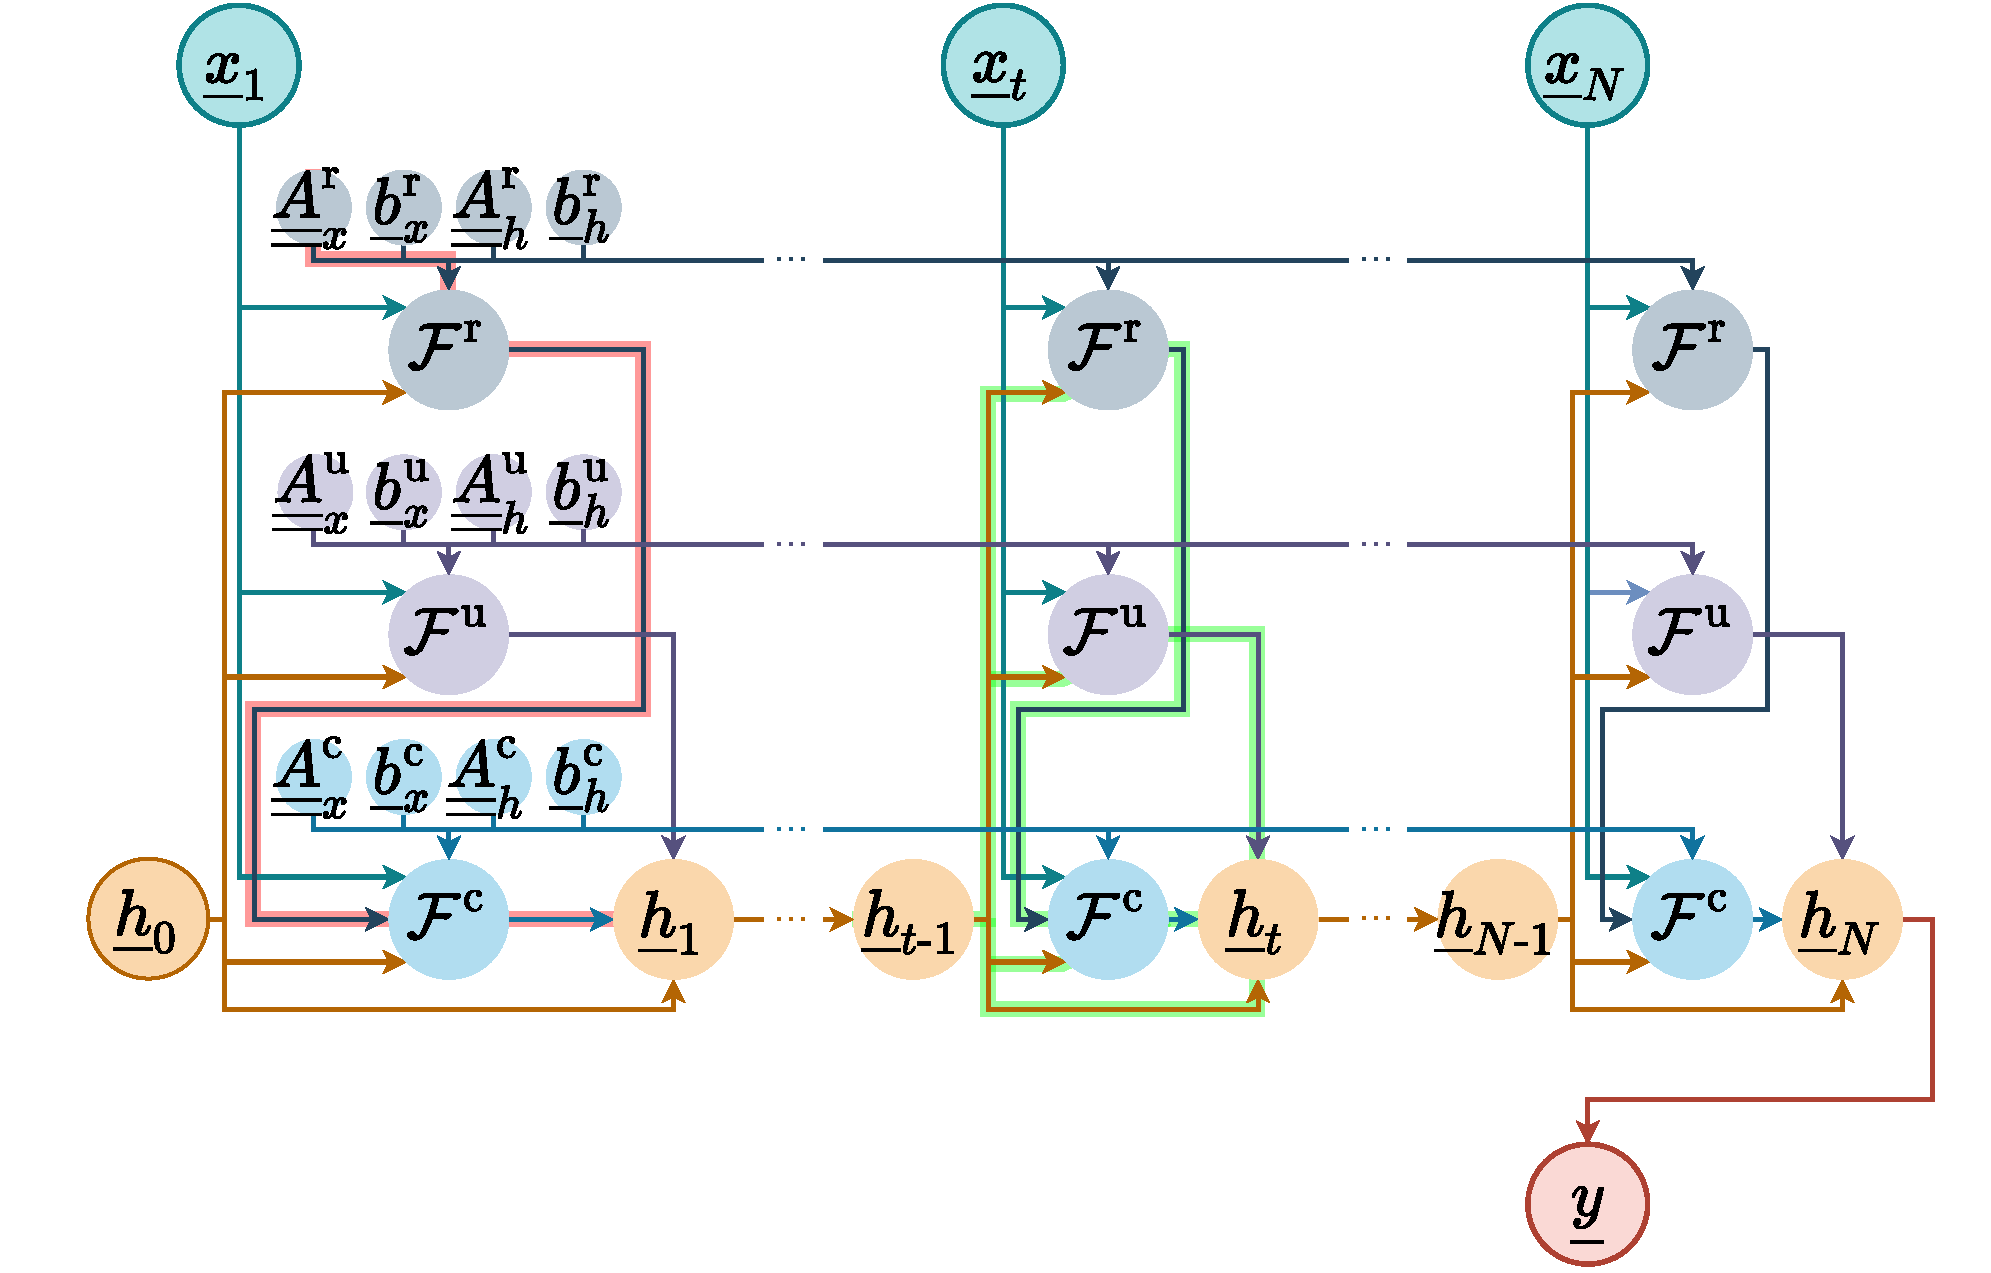
\includegraphics[width=0.9\textwidth]{own/gru_unfolded_intra_inter_paths.drawio.pdf}
    \caption[
        Unfolded GRU in many-to-one mode
    ]{
        Time-unfolded computation graph of a GRU layer in many-to-one mode,
        which maps
        the input sequence $\left(x_t\right)_{t\in\{1,\dots N\}}$ 
        to the single output $\underline y$ equal to the
        hidden state $\underline h_N$ of the last processing step.
        $\mathcal{F}^\text{r}$,
        $\mathcal{F}^\text{u}$
        and $\mathcal{F}^\text{c}$
        (see equ. \ref{eq:gru_reset}, \ref{eq:gru_update} and \ref{eq:gru_candidate})
        are the maps to the
        reset gate, update gate and candidate state, respectively.
        The map 
        $\mathcal{F}^\text{h}$ 
        (see equ. \ref{eq:gru_layer_map_hidden})
        yields the hidden states 
        $\left(h_t\right)_{t\in\{1,\dots N\}}$,
        whereas $\underline h_0$ is initialized.
        The trainable objects
        $\underline{\underline{A}}^\square_\square, \underline{b}^\square_\square$
        of the GRU layer
        are shared across all unfolded time steps.
        The backpropagation path of the intra-gradient with respect to 
        $\underline{\underline{A}}^\text{r}_x$
        (see equ. \ref{eq:gru_grad_intra_hidden_2_Arx}) 
        is highlighted in red for $t=1$.
        The backpropagation path of the inter-gradient 
        (see equ. \ref{eq:gru_grad_inter}) 
        is highlighted in green
        for $t$.
        \label{fig:gru_unfolded}}
\end{figure}
The GRU layer forwards the batches of 
single outputs to the subsequent layer of the ANN.
After passing the output layer of the ANN, the loss
of the batch is computed by averaging the losses of the batch elements
\begin{equation} \label{eq:loss_of_batch}
    L\left(\underline y_1, \dots, \underline y_{N^\text{batch}}\right) 
    = 
    \frac{1}{N^\text{batch}}
    \sum_{i=1}^{N^\text{batch}} L_i \left(\underline y_i\right).
\end{equation}
Gradient-based methods update the trainable parameters 
of the ANN with the goal to minimize the batch loss. 
To do this, they compute the gradients of the batch loss 
with respect to the trainable parameters. 
The update of the trainable parameters of the integrated GRU layer 
complies with
\begin{equation}
    \underset{\Theta}{\mathrm{argmin}}\ 
    L\left(\underline y_1, \dots, \underline y_{N^\text{batch}}\right).
\end{equation}
In conformity with Li \cite{li2016tutorial}, 
BPTT calculates the gradient of the batch loss 
with respect to an element $\theta \in \Theta$ 
in the set of trainable objects (see equ. \ref{eq:gru_params})
\begin{align} \label{eq:gru_grad_loss_2_theta}
    &\frac{\partial}{\partial \theta}
        L\left(\underline y_1, \dots, \underline y_{N^\text{batch}}\right)
    \nonumber \\ & \quad \overset{\textcolor{black}{(1)}}{=}
    \frac{1}{N^\text{batch}}
    \sum_{i=1}^{N^\text{batch}} 
    \frac{\partial}{\partial \theta}
    L_i \left(\underline y_i\right)
    \nonumber \\ & \quad \overset{\textcolor{black}{(2)}}{=}
    \frac{1}{N^\text{batch}}
    \sum_{i=1}^{N^\text{batch}} \left(
        \frac{\partial L_i}{\partial \underline y_i}
        \frac{\partial \underline y_i}{\partial \theta}
    \right)
    \nonumber \\ & \quad \overset{\textcolor{black}{(3)}}{=}
    \frac{1}{N^\text{batch}}
    \sum_{i=1}^{N^\text{batch}} \left[
        \frac{\partial L_i}{\partial \underline y_i}
        \sum_{j=1}^{N^{seq}} \left(
            \frac{\partial  \underline y_i}{\partial \underline h_{j, i}}
            \widehat{ \frac{\partial \underline h_{j, i}}{\partial \theta}}
        \right)
    \right]
    \nonumber \\ & \quad \overset{\textcolor{black}{(4)}}{=}
    \frac{1}{N^\text{batch}}
    \sum_{i=1}^{N^\text{batch}} \left\{
        \frac{\partial L_i}{\partial \underline y_i}
        \sum_{j=1}^{N^{seq}} \left[
            \prod_{k=j+1}^{N^{seq}} \left(
                \frac{\partial \underline h_{k, i}}{\partial \underline h_{k-1, i}}
            \right)
            \widehat{ \frac{\partial \underline h_{j, i}}{\partial \theta}}
        \right]
    \right\}.
    \\[2ex]
        &\textcolor{black}{\text{\footnotesize (1) 
            Batch loss (equ. \ref{eq:loss_of_batch})}} \nonumber \\
        &\textcolor{black}{\text{\footnotesize (2) 
            Chain rule}} \nonumber \\
        &\textcolor{black}{\text{\footnotesize (3) 
            BPTT (gradient $\widehat{\square}$ considers previous hidden states constant)}} \nonumber \\
        &\textcolor{black}{\text{\footnotesize (4) 
            Many-to-one (equ. \ref{equ:gru_output_many_to_one});
            chain rule applied to $\partial \underline y_i / \partial \underline h_{j, i}$}} \nonumber
\end{align}
In the above formula,
the gradient
$\widehat{\partial \underline h_{j, i} / \partial \theta}$
(hereinafter referred to as intra-gradient) 
treats all previous hidden states 
$\underline h_{\tilde j,\dots, i}, \ \tilde j \in \{0, j-1\}$ as constants.
In doing so, the intra-gradient covers the backpropagation path 
from the hidden state 
$\underline h_{j, i}$
to the trainable object 
$\theta$
only within the same time step $j$.
The full gradient covering all backpropagation paths to 
$\theta$, 
connects all intra-backpropagation paths through time to the output 
$\underline y _i$ 
by multiplying the intra-gradients with the corresponding chains 
of time step inter-gradients
$\partial \underline h_{k, i}/\partial \underline h_{k-1, i}$.



The following exemplarily derives the intra-gradient with respect to
$\theta=\underline{\underline{A}}^\text{r}_x$ 
(see fig \ref{fig:gru_unfolded} for the corresponding backpropagation path):
\begin{align} \label{eq:gru_grad_intra_hidden_2_Arx}
    \widehat{\frac{\partial \underline h_{t, i}}{\partial \underline{\underline{A}}^\text{r}_x}}
    &\overset{\textcolor{black}{(1)}}{=}
    \widehat{\frac{\partial}{\partial \underline{\underline{A}}^\text{r}_x}} \left\{
        \left[
            \underline 1 
            -
            \mathcal{F}^\text{u}\left(\chi\right)
        \right]
        \odot
        \mathcal{F}^\text{c} \left(\chi\right)
        +
        \mathcal{F}^\text{u}\left(\chi\right)
        \odot
        \underline h_{t\text -1,i}
    \right\}
    %\nonumber \\ & \quad \overset{\textcolor{black}{(2)}}{=}
    \nonumber \\ &\overset{\textcolor{black}{(2)}}{=}
    \mathrm{diag} \left[
        \underline 1 
        -
        \mathcal{F}^\text{u}\left(\chi\right)
    \right]
    \widehat{
        \frac{\partial \mathcal{F}^\text{c} \left(\chi\right)}
            {\partial \underline{\underline{A}}^\text{r}_x} 
    }
    \\[2ex]
    &\textcolor{black}{\text{\footnotesize (1) 
            Map to hidden state (equ. \ref{eq:gru_layer_current_hidden}, \ref{eq:gru_layer_map_hidden}); 
            $\chi :=  \left(\underline x_{t, i}, \underline h_{t\text{-}1, i}\right)$}} \nonumber \\
    &\textcolor{black}{\text{\footnotesize (2) 
        Sum rule;
    }} \nonumber \\
    &\textcolor{black}{\text{\footnotesize \qquad
        Map to update gate (equ. \ref{eq:gru_update}): 
        $\widehat{\partial \mathcal{F}^\text{u} / \partial \underline{\underline{A}}^\text{r}_x} = 0$ 
    }} \nonumber \\
    &\textcolor{black}{\text{\footnotesize \qquad
        Consider
        $\widehat{\partial \underline h_{t\text -1, i} / \partial \underline{\underline{A}}^\text{r}_x} = 0$;
    }} \nonumber \\
    &\textcolor{black}{\text{\footnotesize \qquad
        Hadamard product of 2 vectors (equ. \ref{eq:hadamard_product_two_vectors})
    }} \nonumber
\end{align}
with
\begin{align} \label{eq:gru_grad_intra_candidate_2_Arx}
    \widehat{
        \frac{\partial \mathcal{F}^\text{c} \left(\chi\right)}
            {\partial \underline{\underline{A}}^\text{r}_x}
    }
    & \overset{\textcolor{black}{(1)}}{=}
    \widehat{
        \frac{\partial}{\partial \underline{\underline{A}}^\text{r}_x} 
    }
    \left\{
        \overset{\scriptscriptstyle \odot}{\tanh} \left[
            \underbrace{
            \underline{\underline A}^\text{c}_{x}
            \underline x_{t,i}
            +
            \underline b^\text{c}_{x}
            +
            \mathcal{F}^\text{r}\left(\underline x_{t, i}, \underline h_{t\text -1, i}\right)
            \odot
            \left(
                \underline{\underline A}^\text{c}_{h}
                \underline h_{t\text -1,i}
                +
                \underline b^\text{c}_{h}
            \right)}_{:=\chi^\text{c}}
        \right]
    \right\}
    \nonumber \\ & \overset{\textcolor{black}{(2)}}{=}
    \mathrm{diag} \left[
        \frac{\partial}{\partial \chi^\text{c}}
        \overset{\scriptscriptstyle \odot}{\tanh} \left(\chi^\text{c}\right)
    \right] 
    \cdot 
    \widehat{
        \frac{\partial \chi^\text{c}}
            {\partial \underline{\underline{A}}^\text{r}_x} 
    }
    \nonumber \\ & \overset{\textcolor{black}{(3)}}{=}
    \mathrm{diag} \left[
        1 - \overset{\scriptscriptstyle \odot}{\tanh}{}^2 \left(\chi^\text{c}\right)
    \right] 
    \cdot
    \mathrm{diag} \left(
        \underline{\underline A}^\text{c}_{h}
        \underline h_{t-1,i}
        +
        \underline b^\text{c}_{h}
    \right)
    \widehat{
        \frac{\partial \mathcal{F}^\text{r}\left(\underline x_{t, i}, \underline h_{t\text -1, i}\right)}
            {\partial \underline{\underline{A}}^\text{r}_x} 
    }
    \\[2ex]
    &\textcolor{black}{\text{\footnotesize (1) 
            Map to candidate state (equ. \ref{eq:gru_candidate}); 
            $\chi :=  \left(\underline x_{t, i}, \underline h_{t\text{-}1, i}\right)$}} \nonumber \\
    &\textcolor{black}{\text{\footnotesize (2) 
        Chain rule;  
    }} \nonumber \\
    &\textcolor{black}{\text{\footnotesize \qquad
        Derivative of element-wise function
        (equ. \ref{eq:derivative_vector_elementwise_applied_function})
    }} \nonumber \\
    &\textcolor{black}{\text{\footnotesize (3) 
        Derivative of tanh (equ. \ref{eq:derivative_tanh}); 
    }} \nonumber \\
    &\textcolor{black}{\text{\footnotesize \qquad
    Hadamard product of 2 vectors (equ. \ref{eq:hadamard_product_two_vectors})
    }} \nonumber
\end{align}
and
\begin{align} \label{eq:gru_grad_intra_reset_2_Arx} 
    \widehat{
        \frac{\partial \mathcal{F}^\text{r}\left(\underline x_{t, i}, \underline h_{t\text -1, i}\right)}
            {\partial \underline{\underline{A}}^\text{r}_x} 
    }
    &\overset{\textcolor{black}{(1)}}{=}
    \widehat{
        \frac{\partial}{\partial \underline{\underline{A}}^\text{r}_x} 
    }
    \left[
        \overset{\scriptscriptstyle \odot}{\sigma} \left(
            \underbrace{
            \underline{\underline A}^\text{r}_{x}
            \underline x_{t,i}
            +
            \underline b^\text{r}_{x}
            +
            \underline{\underline A}^\text{r}_{h}
            \underline h_{t\text -1,i}
            +
            \underline b^\text{r}_{h}}_{:=\chi^\text{r}}
        \right)
    \right]
    \nonumber \\ & \overset{\textcolor{black}{(2)}}{=}
    \mathrm{diag} \left[
        \frac{\partial}{\partial \chi^\text{r}}
        \overset{\scriptscriptstyle \odot}{\sigma} \left(\chi^\text{r}\right)
    \right]
    \cdot
    \widehat{
        \frac{\partial \chi^\text{u}{}}
            {\partial \underline{\underline{A}}^\text{r}_x} 
    }
    \nonumber \\ & \overset{\textcolor{black}{(3)}}{=}
    \mathrm{diag} \left\{
        \overset{\scriptscriptstyle \odot}{\sigma} \left(\chi^\text{r}\right)
        \odot
        \left[
            1 -  \overset{\scriptscriptstyle \odot}{\sigma} \left(\chi^\text{r}\right)
        \right]
    \right\}
    \cdot
    \frac{\partial \underline{\underline A}^\text{r}_{x}\underline x_{t,i}}
        {\partial \underline{\underline{A}}^\text{r}_x} 
        .
    \\[2ex]
        &\textcolor{black}{\text{\footnotesize (1) 
            Map to reset gate (equ. \ref{eq:gru_reset})}} \nonumber \\
        &\textcolor{black}{\text{\footnotesize (2) 
            Chain rule;
        }} \nonumber \\
        &\textcolor{black}{\text{\footnotesize \qquad
            Derivative of element-wise function
            (equ. \ref{eq:derivative_vector_elementwise_applied_function})
        }} \nonumber \\
        &\textcolor{black}{\text{\footnotesize (3) 
            Derivative of sigmoid (equ. \ref{eq:derivative_sigmoid})
        }} \nonumber
\end{align}
For the calculation of the gradient
$\partial \left(\underline{\underline A}^\text{r}_{x}\underline x_{t,i}\right)
        /\partial \underline{\underline{A}}^\text{r}_x
$,
which is a three-dimensional tensor 
of only two-dimensional information content, 
refer to \cite{LearnedMiller}, for example.

As required by equation \ref{eq:gru_grad_loss_2_theta}, 
the following derives the inter-gradient
(see fig \ref{fig:gru_unfolded} for the corresponding backpropagation path):
%$\underline h_{t, i} = 
%\mathcal{F}^\text{h} \left(\underline x_{t, i}, \underline h_{t\text{-}1, i}\right)$
%and 
%$\chi :=  \left(\underline x_{t, i}, \underline h_{t\text{-}1, i}\right)$:
\begin{align} \label{eq:gru_grad_inter}
    \frac{\partial \underline h_{t, i}}{\partial \underline h_{t\text{-}1, i}}
    %\nonumber \\ & \quad \overset{\textcolor{black}{(1)}}{=}
    %\frac{\partial}{\partial \underline h_{t\text{-}1, i}}
    %\mathcal{F}^\text{h} \left(\underline x_{t, i}, \underline h_{t\text{-}1, i}\right)
    %\nonumber \\ & \quad \overset{\textcolor{black}{(1)}}{=}
    &\overset{\textcolor{black}{(1)}}{=}
    \frac{\partial}{\partial \underline h_{t\text{-}1, i}} \left\{
        \left[
            \underline 1 
            -
            \mathcal{F}^\text{u}\left(\chi\right)
        \right]
        \odot
        \mathcal{F}^\text{c} \left(\chi\right)
        +
        \mathcal{F}^\text{u}\left(\chi\right)
        \odot
        \underline h_{t\text -1,i}
    \right\}
    %\nonumber \\ & \quad \overset{\textcolor{black}{(2)}}{=}
    \nonumber \\ &\overset{\textcolor{black}{(2)}}{=}
    \frac{\partial}{\partial \underline h_{t\text{-}1, i}} \left\{
        \left[
            \underline 1 
            -
            \mathcal{F}^\text{u}\left(\chi\right)
        \right]
        \odot
        \mathcal{F}^\text{c} \left(\chi\right)
    \right\}
    +
    \frac{\partial}{\partial \underline h_{t\text{-}1, i}} \left\{
        \mathcal{F}^\text{u}\left(\chi\right)
        \odot
        \underline h_{t-1,i}
    \right\}
    %\nonumber \\ & \quad \overset{\textcolor{black}{(3)}}{=}
    \nonumber \\ & \overset{\textcolor{black}{(3)}}{=}
    - \mathrm{diag}\left[\mathcal{F}^\text{c} \left(\chi\right)\right] 
    \frac{\partial \mathcal{F}^\text{u}\left(\chi\right)}
        {\partial \underline h_{t\text{-}1, i}}
    +
    \mathrm{diag} \left[
        \underline 1 
        -
        \mathcal{F}^\text{u}\left(\chi\right)
    \right]
    \frac{\partial \mathcal{F}^\text{c} \left(\chi\right)}
        {\partial \underline h_{t\text{-}1, i}}
    \nonumber \\ &\qquad +
    \mathrm{diag} \left(\underline h_{t-1,i}\right)
    \frac{\partial \mathcal{F}^\text{u}\left(\chi\right)}
        {\partial \underline h_{t\text{-}1, i}}
    +
    \mathrm{diag} \left[
        \mathcal{F}^\text{u}\left(\chi\right)
    \right].
    \\[2ex]
    &\textcolor{black}{\text{\footnotesize (1) 
            Map to hidden state (equ. \ref{eq:gru_layer_current_hidden}, \ref{eq:gru_layer_map_hidden}); 
            $\chi :=  \left(\underline x_{t, i}, \underline h_{t\text{-}1, i}\right)$}} \nonumber \\
    &\textcolor{black}{\text{\footnotesize (2) 
        Sum rule
    }} \nonumber \\
    &\textcolor{black}{\text{\footnotesize (3) 
        Differentiation of Hadamard product of 2 vectors 
        (equ. \ref{eq:differentiation_hadamard_product_two_vectors})
    }} \nonumber
\end{align}
with
\begin{align} \label{eq:gru_grad_update_2_previous_hidden} 
    \frac{\partial
    \mathcal{F}^\text{u} \left(\underline x_{t, i}, \underline h_{t\text{-}1, i}\right)
    }{\partial \underline h_{t\text{-}1, i}}
    &\overset{\textcolor{black}{(1)}}{=}
    \frac{\partial}{\partial \underline h_{t\text{-}1, i}}
    \left[
        \overset{\scriptscriptstyle \odot}{\sigma} \left(
            \underbrace{
            \underline{\underline A}^\text{u}_{x}
            \underline x_{t,i}
            +
            \underline b^\text{u}_{x}
            +
            \underline{\underline A}^\text{u}_{h}
            \underline h_{t\text -1,i}
            +
            \underline b^\text{u}_{h}}_{:=\chi^\text{u}}
        \right)
    \right]
    \nonumber \\ & \overset{\textcolor{black}{(2)}}{=}
    \mathrm{diag} \left[
        \frac{\partial}{\partial \chi^\text{u}}
        \overset{\scriptscriptstyle \odot}{\sigma} \left(\chi^\text{u}\right)
    \right]
    \cdot \frac{\partial}{\partial \underline h_{t\text{-}1, i}} \chi^\text{u}{}
    \nonumber \\ & \overset{\textcolor{black}{(3)}}{=}
    \mathrm{diag} \left\{
        \overset{\scriptscriptstyle \odot}{\sigma} \left(\chi^\text{u}\right)
        \odot
        \left[
            1 -  \overset{\scriptscriptstyle \odot}{\sigma} \left(\chi^\text{u}\right)
        \right]
    \right\}
    \cdot \underline{\underline A}^\text{u}_{h},
    \\[2ex]
        &\textcolor{black}{\text{\footnotesize (1) 
            Map to update gate (equ. \ref{eq:gru_update})}} \nonumber \\
        &\textcolor{black}{\text{\footnotesize (2) 
            Chain rule;
        }} \nonumber \\
        &\textcolor{black}{\text{\footnotesize \qquad
            Derivative of element-wise function
            (equ. \ref{eq:derivative_vector_elementwise_applied_function})
        }} \nonumber \\
        &\textcolor{black}{\text{\footnotesize (3) 
            Derivative of sigmoid (equ. \ref{eq:derivative_sigmoid})
        }} \nonumber
\end{align}
and
\begin{align} \label{eq:gru_grad_candidate_2_previous_hidden}
    &\frac{\partial}{\partial \underline h_{t\text{-}1, i}}
    \mathcal{F}^\text{c}\left(\underline x_{t, i}, \underline h_{t\text -1, i}\right)
    \nonumber \\ & \quad \overset{\textcolor{black}{(1)}}{=}
    \frac{\partial}{\partial \underline h_{t\text{-}1, i}}
    \left\{
        \overset{\scriptscriptstyle \odot}{\tanh} \left[
            \underbrace{
            \underline{\underline A}^\text{c}_{x}
            \underline x_{t,i}
            +
            \underline b^\text{c}_{x}
            +
            \mathcal{F}^\text{r}\left(\underline x_{t, i}, \underline h_{t\text -1, i}\right)
            \odot
            \left(
                \underline{\underline A}^\text{c}_{h}
                \underline h_{t\text -1,i}
                +
                \underline b^\text{c}_{h}
            \right)}_{:=\chi^\text{c}}
        \right]
    \right\}
    \nonumber \\ & \quad \overset{\textcolor{black}{(2)}}{=}
    \mathrm{diag} \left[
        \frac{\partial}{\partial \chi^\text{c}}
        \overset{\scriptscriptstyle \odot}{\tanh} \left(\chi^\text{c}\right)
    \right] 
    \cdot 
    \frac{\partial}{\partial \underline h_{t\text{-}1, i}} \chi^\text{c}
    \nonumber \\ & \quad \overset{\textcolor{black}{(3)}}{=}
    \mathrm{diag} \left[
        1 - \overset{\scriptscriptstyle \odot}{\tanh}{}^2 \left(\chi^\text{c}\right)
    \right] 
    \nonumber \\ &\quad \quad  \cdot
    \left\{
        \mathrm{diag} \left(
            \underline{\underline A}^\text{c}_{h}
            \underline h_{t-1,i}
            +
            \underline b^\text{c}_{h}
        \right)
        \frac{\partial \mathcal{F}^\text{r}\left(\underline x_{t, i}, \underline h_{t\text -1, i}\right)}
        {\partial \underline h_{t\text -1, i}}
        +
        \mathrm{diag}\left[
            \mathcal{F}^\text{r}\left(\underline x_{t, i}, \underline h_{t\text -1, i}\right)
        \right]
        \underline{\underline A}^\text{c}_{h}
    \right\}.
    \\[2ex]
        &\textcolor{black}{\text{\footnotesize (1)
            Map to candidate state (equ. \ref{eq:gru_candidate})
        }} \nonumber \\
        &\textcolor{black}{\text{\footnotesize (2) 
            Chain rule of differentiation;  
        }} \nonumber \\
        &\textcolor{black}{\text{\footnotesize \qquad 
            Derivative of function applied element-wise on vector
            (equ. \ref{eq:derivative_vector_elementwise_applied_function})
        }} \nonumber \\
        &\textcolor{black}{\text{\footnotesize (3) 
            Derivative of hyperbolic tangent (equ. \ref{eq:derivative_tanh}); 
        }} \nonumber \\
        &\textcolor{black}{\text{\footnotesize \qquad
            Differentiation of Hadamard product of 2 vectors 
            (equ. \ref{eq:differentiation_hadamard_product_two_vectors})
        }} \nonumber
\end{align}
as well as (same structure as in equ. \ref{eq:gru_grad_update_2_previous_hidden})
%The in equation \ref{eq:gru_grad_candidate_2_previous_hidden} 
%required gradient of the current reset gate
%with respect to the previous hidden state shares the same structure
%with the gradient of equation \ref{eq:gru_grad_update_2_previous_hidden} 
%and is hence derived as
\begin{align}
    \frac{\partial}{\partial \underline h_{t\text{-}1, i}}
    \mathcal{F}^\text{r} \left(\underline x_{t, i}, \underline h_{t\text{-}1, i}\right)
    &=
    \mathrm{diag} \left\{
        \overset{\scriptscriptstyle \odot}{\sigma} \left(\chi^\text{r}\right)
        \odot
        \left[
            1 -  \overset{\scriptscriptstyle \odot}{\sigma} \left(\chi^\text{r}\right)
        \right]
    \right\}
    \cdot \underline{\underline A}^\text{r}_{h}
    \nonumber \\
    \text{with } \chi^\text{r} & :=
    \underline{\underline A}^\text{r}_{x}
            \underline x_{t,i}
            +
            \underline b^\text{r}_{x}
            +
            \underline{\underline A}^\text{r}_{h}
            \underline h_{t\text -1,i}
            +
            \underline b^\text{r}_{h}.
\end{align}
The above derivations revert to the following equations.
Equations (4.5.73) and (4.5.17) of Abramowitz and Stegun \cite{D.1966}
yield the derivative of the hyperbolic tangent as
\begin{equation} \label{eq:derivative_tanh}
    \frac{\text d}{\text d x} \tanh (x) = 1 - \tanh^2 (x).
\end{equation}
The derivative of the sigmoid function (e.g., \cite{Minai1993}) is
\begin{equation} \label{eq:derivative_sigmoid}
    \frac{\text d}{\text d x} \sigma \left(x\right) 
    = 
    \sigma \left(x\right) 
    \left[
        1 - \sigma \left(x\right)
    \right].
\end{equation}
The Hadamard product of two vectors \cite{Brookes2020} equates to the 
matrix product of a diagonal matrix and a vector 
\begin{equation} \label{eq:hadamard_product_two_vectors}
    \underline x_1 \odot \underline x_2 
= 
    \mathrm{diag} \left(\underline x_1\right) \underline x_2 
=   
    \mathrm{diag} \left(\underline x_2\right) \underline x_1.
\end{equation}
Applying the product rule of differentiation 
yields the derivative of the Hadamard product of two vectors
\begin{equation} \label{eq:differentiation_hadamard_product_two_vectors}
    \frac{\partial}{\partial t} \left(
        \underline x_1 \odot \underline x_2 
    \right)
    =   
    \mathrm{diag} \left(\underline x_2\right)
    \frac{\partial \underline x_1}{\partial t} 
    +
    \mathrm{diag} \left(\underline x_1\right)
    \frac{\partial \underline x_2}{\partial t}.
\end{equation}
The derivative of a function
$f:\mathbb{R}\rightarrow\mathbb{R}$ applied element-wise to a vector $\underline x$
is the diagonal matrix built from the derivative of the function applied element-wise on the vector
\begin{equation} \label{eq:derivative_vector_elementwise_applied_function}
        \frac{\partial}{\partial \underline x} 
        \overset{\scriptscriptstyle \odot}{f} \left(
                \underline x
            \right)
    =
        \mathrm{diag} \left[
            \overset{\scriptscriptstyle \odot}{f'}  \left(
                \underline x
            \right)
        \right].
\end{equation}
The calculation of the differential of the function yields the above statement
\begin{align}
    &\frac{\text d}{\text d \underline x}
    \overset{\scriptscriptstyle \odot}{f} \left(
        \underline x
    \right)
    \cdot \text d \underline x
\overset{\textcolor{black}{(1)}}{=}
    \text d 
    \overset{\scriptscriptstyle \odot}{f} \left(
        \underline x
    \right)
\overset{\textcolor{black}{(2)}}{=}
    \left[
        \overset{\scriptscriptstyle \odot}{f'}  \left(
            \underline x
        \right)
    \right]
    \odot \text d \underline x
\overset{\textcolor{black}{(3)}}{=}
    \mathrm{diag} \left[
        \overset{\scriptscriptstyle \odot}{f'}  \left(
            \underline x
        \right)
    \right]\cdot
    \text d \underline x.
    \\[2ex]
        &\quad\textcolor{black}{\text{\footnotesize (1) Relation of differential and derivative}} \nonumber \\
        &\quad\textcolor{black}{\text{\footnotesize (2) Chain rule element-wise applied}} \nonumber \\
        &\quad\textcolor{black}{\text{\footnotesize (3) Hadamard product of 2 vectors (equ. \ref{eq:hadamard_product_two_vectors})}}
\end{align}